%!TEX root = ../Thesis.tex

This section will focus on basic grid-based path-planning algorithms used mostly in single-agent scenarios. Those algorithms are usually graph-based and represent a map as a set of vertices and edges. The graph can be either undirected or directed, depending on whether the agent is allowed to move in both or in just one direction between vertices\cite{basic_algorithms}. Only three algorithms will be discussed in this section: Dijkstra's Algorithm, A* Algorithm, and BFS algorithm, as they are useful for further understanding of more complex algorithms. A diagram explaining the general approach for graph-based path planning is shown in figure \ref{fig:simple_path_planning}. 

\begin{figure}[H]
    \centering
    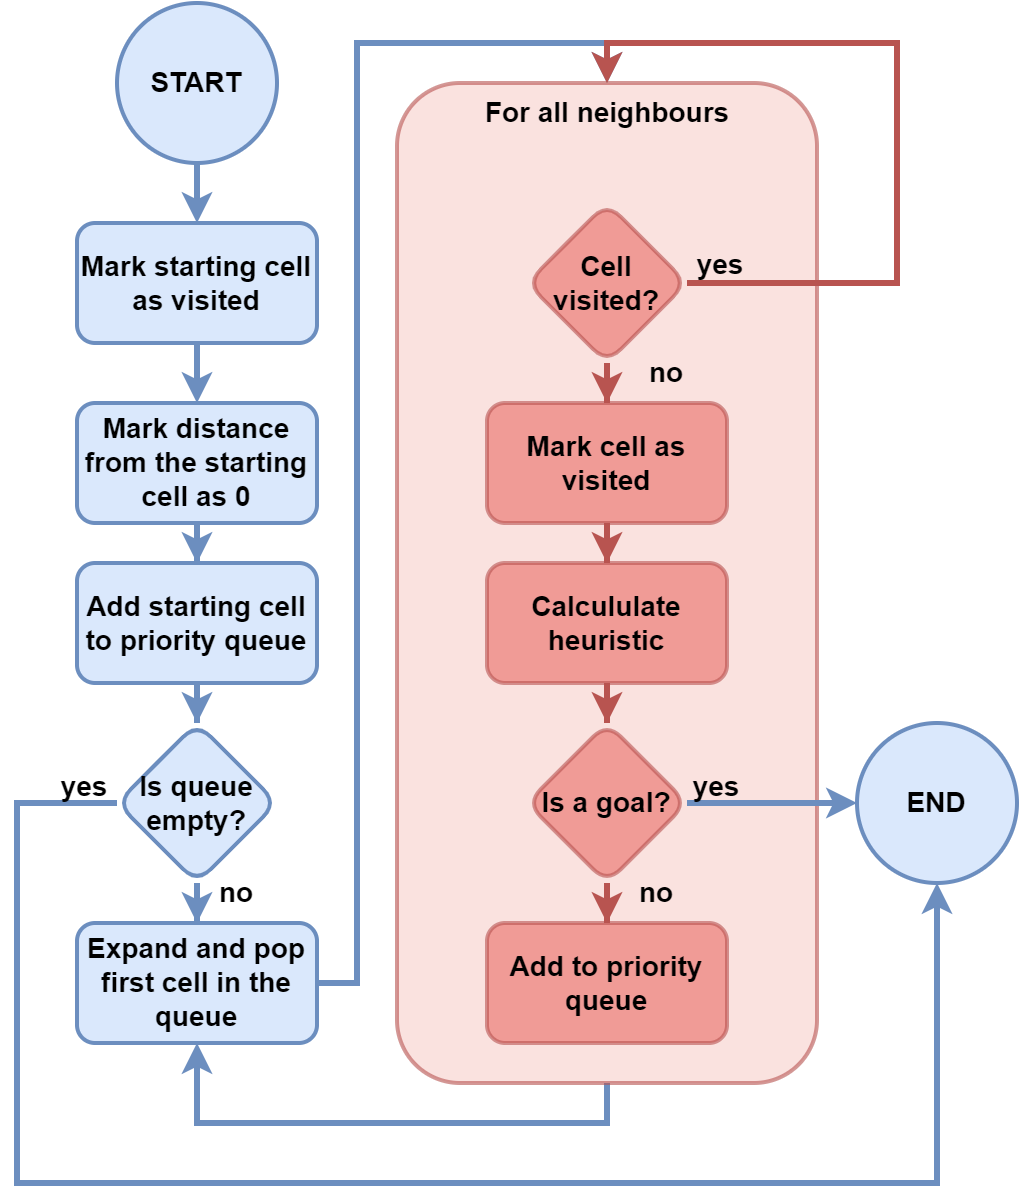
\includegraphics[width=0.7\textwidth]{pictures/simple_algos.png}
    \caption{General approach for graph-based path planning algorithms. }
    \label{fig:simple_path_planning}
\end{figure}


\subsection{Dijkstra's Algorithm}
Dijkstra's Algorithm assigns a minimal length(edge value - g(n)) from a starting point for every vertex in a graph, initially starting point has a length of 0 assigned, and others have infinity. For each step of the algorithm, new vertices are expanded(the ones which are neighbors of the one with the lowest length from start) and marked as visited. If all vertices are visited or the goal is reached then the algorithm terminates, otherwise continue expansion\cite{basic_algorithms}. The algorithm is guaranteed to find the shortest path from the starting point to the goal, as long as none of the edges have a negative cost\cite{basic_2}.

\subsection{Greedy Best-First-Search}
This algorithm takes an opposite approach to the previous one. Instead of exploring nodes with the shortest distance from the start, it tries to explore the ones closest to the goal, using the heuristic function - h(n). This is what makes the search algorithm 'greedy' as it wants to reach the goal as quickly as possible, not considering obstacles in a way. It is a fast algorithm, but the routes found are often sub-optimal.

\subsection{A* Algorithm}
A* is the most popular choice for pathfinding, because of its simplicity and robustness. It has also many advanced extensions used in a multi-agent systems approach. It works very similarly to Dijkstra's algorithm, except it is using heuristics to guide itself. It combines the information about the distance from the start - g(n) and the heuristic function which is usually a distance to a goal - h(n). In each iteration, it examines the node that has the lowest sum of g(n) + h(n)\cite{basic_2}.

The behavior of A* algorithm will vary, depending on the heuristic function that is being used. It is usually faster than Dijkstra when finding a solution, but a result can be sub-optimal so it is a challenge to balance those two.
